\documentclass{article}
\usepackage{enumitem}
\usepackage{graphicx}
\graphicspath{{images/}}

\begin{document}
\begin{enumerate}[label=\textbf{\Alph*.}]
	\item For degree n, how many additions and how many multiplications does this
	code perform? \\
	Both operation perform n times.
	\item . \\
	\begin{figure}[h]
		\centering
		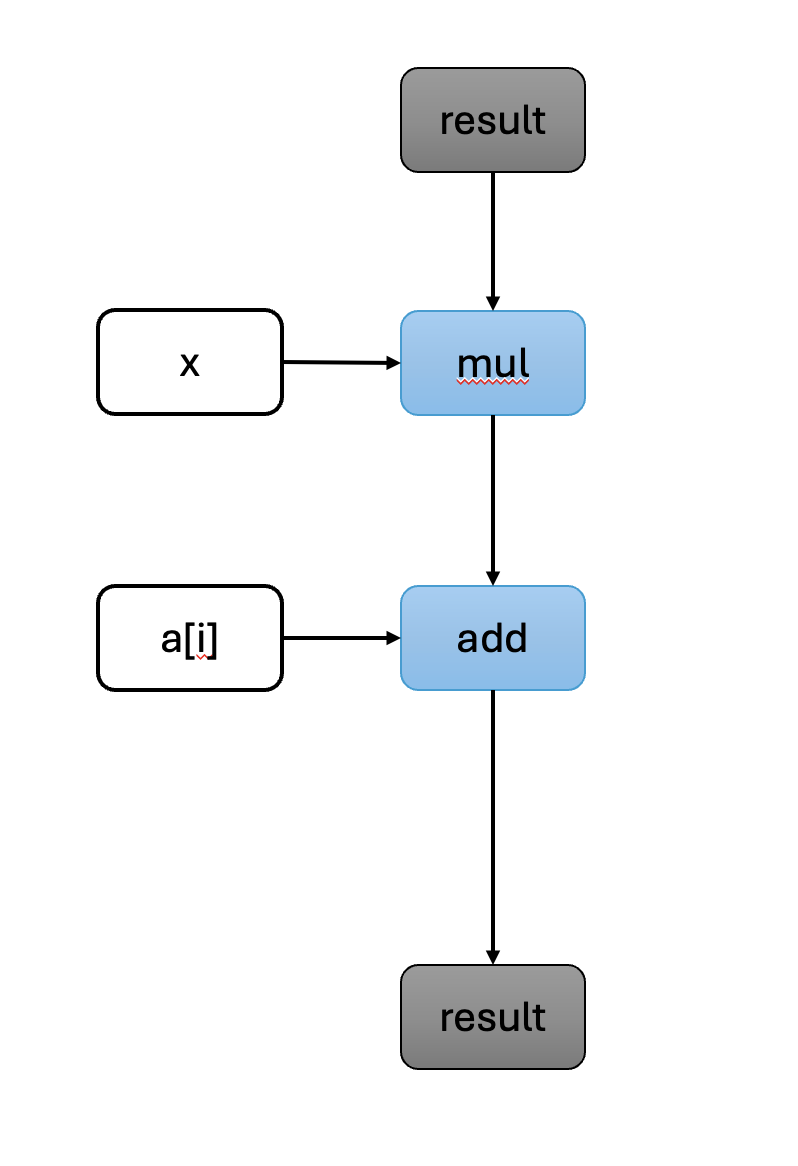
\includegraphics[width=0.75\textwidth]{fig1}
	\end{figure} \\
	Floating point multiplication will use 5 clock cycle and floating
	point add will use 3 clock cycle. And this two operation cannot
	perform in parallel.
	\item . \\
	In 5.5 this the multiplication can be done in parallel with the
	addition, because the operand in the multiplication is not
	dependent with the result in last iteration.
\end{enumerate}
\end{document}
